\chapter{Optical Microcavity}
%Descrição teórica do caso geral. O objetivo aqui é deixa claro o conceito de modos, modo azimutal, dispersão da cavidade, autovalor e autovetor. Assim, quando eu falar sobre os modos acoplados a ideia de perturbação no autoestado fica mais facil de entender. 
%
%Talvez uma descrição mais detalhada sobre a fase acumulada ajude na hora de falar sobre o phase matching, por outro lado pode ser uma descrição fundamental demais. 
%
%Também faz parte dessa sessão o experimento de caracterização. Acho que não tem muita necessidade de entrar em detalhes aqui e, se for o caso, podemos aproveitar o apêndice para informações mais técnicas (como fabricação do taper por exemplo). 

As seen in last Chapter, nonlinear phenomena demand high electric fields when compared with the atomic electric field. Just in order to compare, a silicon atom (note that I used a silicon atom as example just to to simplify the atomic model, my cavities aren't build in silicon) has a atomic radius ($\rho_0$) of about $210$~pm and the atomic number of 14, with enable us to estimate   
\begin{equation}
   E_\text{atomic} = -\frac{1}{4 \pi \epsilon0}\frac{Z e^-}{\rho_0^2} %\approx 1.4\times10^{-9}\frac{Z}{\rho_0^2} 
    \approx 4.5\times10^{11}\text{V/m}.
\end{equation}

The approach we applied in order to reach some comparable electric field is confine it in a optical cavity. By recycle the photons trapped inside and confine they in a small space, the optical cavity enable to reach a high circulating power in a small effective area, lead to a high intensity hence high electric field. 

A typical optical mode, for a Whispering Gallery Mode (don't worry, it will be clear further) cavity with about $100~\mu$m of radius, presents a effective area ($A$) of around $2~\mu$m and enable circulating power ($P$) as high as $1$~KW. We can estimate the electric field confined in a silicon cavity (just to compare) as 
\begin{equation}
    E_\text{confined} = \sqrt{\frac{2}{c\text{n}\epsilon_0}\frac{P}{A}} \approx 3 \times 10^8\text{V/m}.
\end{equation}
\nomenclature{$c$}{Speed of Light in Vacuum}
Where $\text{n}$ is the refraction index for silicon. 

Lets first introduce the theory for uncoupled modes, where I describe the behavior of any single mode of the cavity. Them we consider the nonlinearity of the medium to describe the coupled mode theory. 

\section{Single Mode Theory}

Considering a slowly varying envelop for the electromagnetic field, it is possible to write they as separable time and space function
\begin{equation}
    \genfrac{}{}{0 pt}{}{\vec{E}(\vec{r},t)}{\vec{H}(\vec{r},t)} = \sum_j a_j(t)\genfrac{(}{)}{0 pt}{}{\vec{e}_j(\vec{r})}{\vec{h}_j(\vec{r})}.
    \label{eq:general_mode}
\end{equation}
Each pair ($\vec{e_j},\vec{h_j}$) describe the spatial distribution of the $j$th\footnote{$j$ are a label and can assume any form, not necessary numerical} unperturbed harmonic mode of frequency $\omega_j$, hence 

\begin{equation}
    \nabla \times \genfrac{(}{)}{0 pt}{}{\vec{e}_j(\vec{r})}{\vec{h}_j(\vec{r})} = i\omega_j \genfrac{(}{)}{0 pt}{}{\mu_0\vec{h}_j(\vec{r})}{-\n^2\epsilon_0\vec{e}_j(\vec{r})}.
    \label{eq:spatial_distribution}
\end{equation}

Applying the Eq~\ref{eq:general_mode} and Eq~\ref{eq:spatial_distribution} in the Maxwell's equations, Eq~\ref{eq:max_eq}c and Eq~\ref{eq:max_eq}d, we get

\begin{subequations}
    \begin{alignat}{2}
        &\sum_j \left(\dot{a}_j + i \omega_j a\right) \mu_0 \vec{h}_j &&= 0,\\
        &\sum_j \left(\dot{a}_j + i \omega_j a\right) \text{n}^2\epsilon_0 \vec{e}_j &&= -\frac{\partial}{\partial t}\vec{P}^{NL}.
    \end{alignat}
\end{subequations}

Calculating the expectation, borrowing Dirac's notation, normalized by the energy stored in each mode, we them have 
\begin{equation}
    \dot{a}_j + i \omega_j a = -\frac{\braket{\vec{e}_j|\partial_t\vec{P}^{NL}}}{2\epsilon_0\bra{\vec{e}_j}\text{n}^2\ket{\vec{e}_j}}.
    \label{eq:rate_equation_1}
\end{equation}
%(\bra{\vec{h}}\mu_0\ket{\vec{h}}+\bra{\vec{e}_j}\epsilon_0\text{n}^2\ket{\vec{e}_j})
%For solve the equations one must solve it therm by therm, which lead us to the rate equation for the amplitude of the $j$th mode
%\begin{equation}
%    \dot{a}_j + i \omega_j a = 0.
%    \label{eq:rate_equation_1}
%\end{equation}
%wheres we normalized in suck way that $|a_j|^2$ give the total energy stored in the $j$th mode.

In order to compare our model with a real system, we shall introduce losses and source, as long some know phenomena, in Eq~\ref{eq:rate_equation_1}; We going to do both phenomenologically.

Including a non-vanishing imaginary part for the permittivity $\epsilon$. Moreover, a source can be included as a combination in current and charge densities in Maxwell's equations, which is analogous to include a polarization term, $\vec{P}_{in}$, to the total polarization. The time dependence of $\vec{P}_{in}$ has to do only with the source, being independent of the intracavity fields.

This step introduce some extra terms in the Eq~\ref{eq:rate_equation_1}, which results
\begin{equation}
    \dot{a}_j = -\left(i\omega_j +\frac{\kappa_j}{2}\right)a_j -\frac{\braket{\vec{e}_j|\partial_t\vec{P}^{NL}}}{2\epsilon_0\bra{\vec{e}_j}\text{n}^2\ket{\vec{e}_j}}+\frac{\braket{\vec{e}_j|\partial_t\vec{P}_{in}}}{\bra{\vec{e}_j}\text{n}^2\ket{\vec{e}_j}}.
\end{equation}
Wheres $\kappa_j = \kappa^{(i)}_j+\kappa^{(e)}_j$ are the total loss, composed by the intrinsic loss, suck material absorption and scattering loss, and couple loss due to coupling with the source. 

Finally, from input-output theory, it can be show that the feeding term can be written as $\sqrt{\kappa^{(e)}_j}a_{in}(t)$, where $|a_{in}|^2$ gives the pump power. Beside that, for our first analysis, we will consider that the nonlinear therm is small enough to be disregarded. This trick enable us to treat separately the temporal and spatial behavior of the optical modes. 

\subsection{Temporal Equations}

To describe the temporal evolution of the confined modes, we use the rate equation can be rewrite as 
\begin{equation}
    \dot{a}_j = -\left(i\omega_j +\frac{\kappa_j}{2}\right)a_j +\sqrt{\kappa^{(e)}_j}a_{in}(t).
    \label{eq:rate_equation2}
\end{equation} 

In typical laboratory condition, $a_{in}(t)$ correspond to a narrow spectral distribution centered at frequency $\omega_L$. Its makes possible to rewrite Eq~\ref{eq:rate_equation2} in a rotating reference frame that turns the source terms into a constant by interchange $a_j \rightarrow a_je^{-i\omega_Lt}$
\begin{equation}
    \dot{a}_j = -\left(i\Delta_j +\frac{\kappa_j}{2}\right)a_j +\sqrt{\kappa^{(e)}_j}a_{in}.
    \label{eq:rate_equation_unperturbed}
\end{equation}
\nomenclature{$\kappa$}{Total Cavity Loss}
\nomenclature{$\kappa^{(i)}$}{Intrinsic Cavity Loss}
\nomenclature{$\kappa^{(e)}$}{Coupling Cavity Loss}
\nomenclature{$\Delta$}{Laser Detuning}


where $\Delta_j = \omega_j - \omega_L$ is called the detuning.
\begin{figure}[t!]
    \centering
    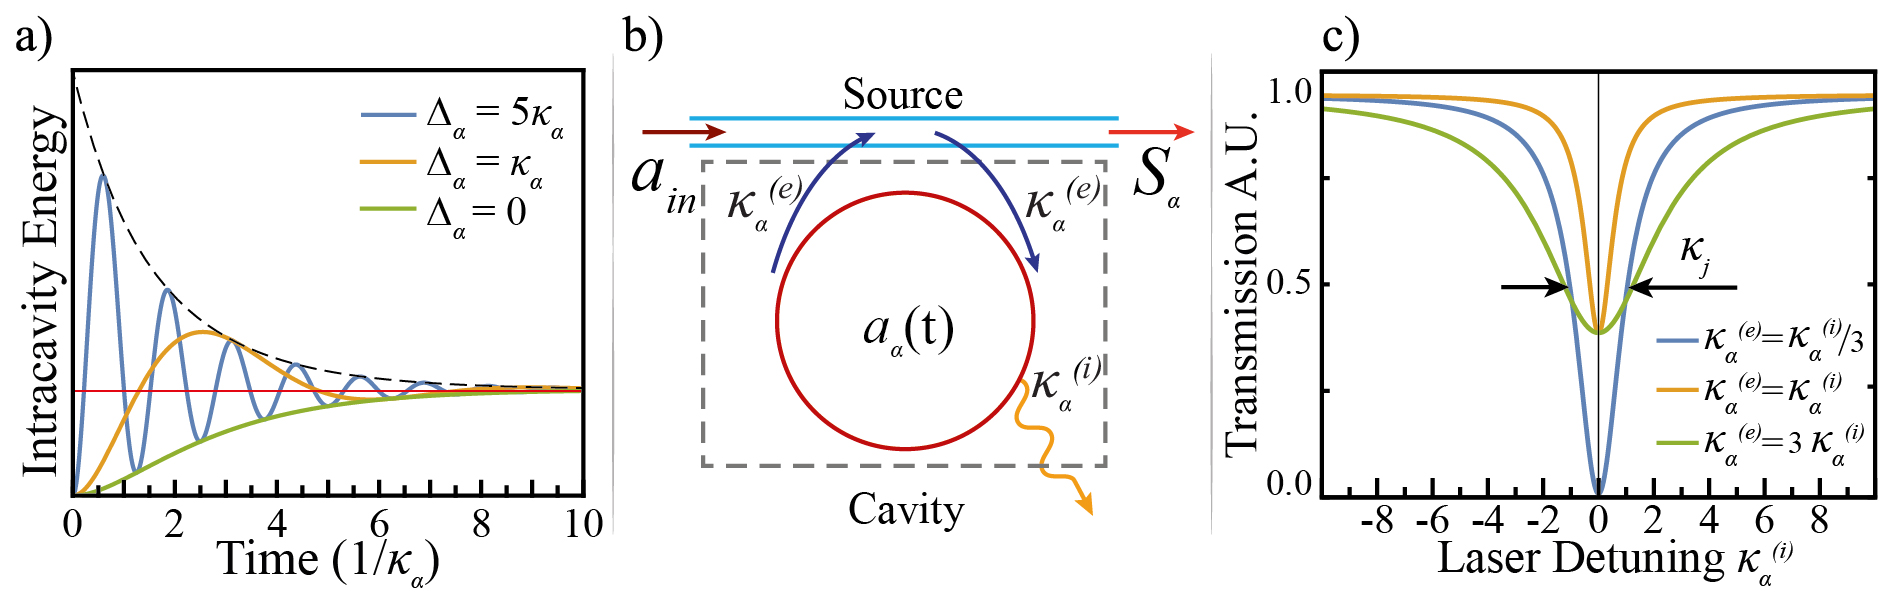
\includegraphics[width = 16cm]{Dissertation_rate_equation.jpg}
    \caption{Caption}
    \label{fig:rate_equations_single_mode}
\end{figure}
A Eq~\ref{eq:rate_equation_unperturbed} accepts harmonic solutions with frequency $\Delta_j$. Nevertheless these solutions decay, with a  $\kappa_j$ rate, into a steady state solution. We usually operates the system in a time scale much larger than $\kappa^{-1}$, thus we consider just the steady state solution. 

We have already introduced the required formalism to describe our problem, now I want you to have a more pictorial, although very useful, view of it. 

Lets consider our system composed by a optical cavity and a source. This cavity have a optical mode with amplitude $a_j$, and present intrinsic loss $\kappa_j^{(i)}$ due scattering and absorption. The source carry a input wave $a_{in}$ at frequency $\omega_L$ which couple with the cavity at an $\kappa_j^{(e)}$ rate, the optical mode couple back with the source at the same frequency, in such way that this couple is seen as a loss channel. The outgoing wave, defined as $S_j$, carry information about the source and the optical mode, in this way
\begin{equation}
    S_j = a_{in} - \sqrt{2 \kappa_j^{(e)}}a_j.
\end{equation}
For the steady state solution, $\dot{a} = 0$, which lead us to define the transmission of the cavity as
\begin{equation}
    T = \left|\frac{S_j}{a_{in}}\right|^2 = \frac{\left(\kappa_j^{(i)} -\kappa_j^{(e)}\right)^2 + (2\Delta_j)^2}{\left(\kappa_j^{(i)} +\kappa_j^{(e)}\right)^2 + (2\Delta_j)^2}.
    \label{eq:single_mode_transmission}
\end{equation}

Typically, the experiment are made by sweep the source frequency. The ration between the intrinsic loss and the coupling loss define the regime of the system; under coupled, for $\kappa_j^{(e)} < \kappa_j^{(i)}$, critical coupled, for $\kappa_j^{(e)} = \kappa_j^{(i)}$, and over coupled, for $\kappa_j^{(e)} > \kappa_j^{(i)}$. 

As the capacity of recycle photons inside the optical cavity is a important feature, we should use a value to determine how efficiently our cavity storage energy. For this purpose we define the Finesse as the ratio between the mean lifetime of the photon inside the cavity and the round trip time, or in function of measurable parameters 
\begin{equation}
    \mathcal{F} = \frac{\text{Mean Lifetime}}{\text{Round Trip Time}} = \frac{FSR_j}{\kappa_j}.
\end{equation}
\nomenclature{$\mathcal{F}$}{Finesse}
Where $FSR_j$ is the Free Spectral Range of the $j$th mode.

However, for our system this two values (the round trip time and the mean lifetime) are coupled, in the sense that we aren't able to increase or decrease the round trip time without affect the mean lifetime, hence we define the Quality factor ($Q$) as the ration between the frequency of the mode ($\omega_j$) and the bandwidth ($\kappa_j$) to determine the efficiency of our cavity to store energy. 

In order to better understand the concept of Free Spectral Range and how do it lead us to the round trip time I must develop the spatial treatment of the modes. 

\subsection{Spatial Equations}

Initially lets consider a propagating wave at frequency $\omega$. From the Maxwell's equations it is possible to write
\begin{subequations}
    \begin{alignat}{2}
    &\nabla^2\vec{h}_j+\beta^2n^2\vec{h}_j &&= \nabla(\nabla\cdot\vec{h}_j),\\
    &\nabla^2\vec{e}_j+\beta^2n^2\vec{e}_j &&= \nabla(\nabla\cdot\vec{e}_j).
    \end{alignat}
    \label{eq:wave_eq_full}
\end{subequations}
Here I defined $\beta = \omega/c$, where $c$ is the speed of light in the vacuum. As the medium that we are interested presents uniform refraction index, the right side of the equation are null. 

We shall assume that the solution is a wave that propagate in $z$ direction with the form $e^{ik_jz}$, hence the Eq~\ref{eq:wave_eq_full} can be rewrite as 

\begin{subequations}
    \begin{alignat}{2}
    &\nabla_t^2\vec{h}_j+(\beta^2n^2-k_j^2)\vec{h}_j &&=0,\\
    &\nabla_t^2\vec{e}_j+(\beta^2n^2-k_j^2)\vec{e}_j &&=0.
    \end{alignat}
    \label{eq:wave_eq}
\end{subequations}
Where $\nabla_t^2 = \nabla^2 - \partial^2/\partial z^2$.

It might be have been overlooked, but the Eq~\ref{eq:wave_eq} is a system with 6 equation; one for which field in each coordinate. The solution for this set of equation with boundary condition define the optical modes of our problem. To solve this equations we must apply consideration about symmetry, however we use numerical methods to solve it. We will use the commercial software COMSOL\regmark, in Appendix~\ref{app:Comsol_Solution} we explained step by step how this solutions are done. 

Until now we have talk about generic electromagnetic modes, with no spatial boundary condition, in order to define them we must define the geometry of our cavity. Our device are based in disk microcavities, as show in Fig~%\ref{}
, this kind of resonator presents the so called Whispering Gallery Modes (WGM), due to cylindrical symmetry. In order to archive high life time of the photons inside the cavity we use a wedge cavity, the angle present at edge makes the electric field to be less perpendicular to the surface leading to lower loss to scattering, moreover the fabrication process have a important role in here, as we shall see below. 

The boundary condition lead to the characteristic equation in the form 
\begin{equation}
    F(k_r,k_\theta,k_z) = 0.
\end{equation}
The set of constants, $k_r,k_\omega,k_z$, that solve this equation define a single mode. As the mode is confined in a region, we can correlate this constants, that can assume any complex value, to integer with spatial representation.

The WGM are labeled in the format TExy and TMxy modes, where x and y are integer correlated with $k_r$ and $k_z$, respectively. Beside that, given a TExy (TMxy) mode it can have several values of $m$, which is a integer correlated with $k_\theta$, it also define the family of the mode. The spatial mean of the constants are show in Fig~%\ref{}
. Just to clarify the nomenclature adopted in this dissertation, henceforward the term '$j$th mode' are applied for a TExy or TMxy mode with any value of $m$. 

Now we have enough knowledge to understand how to experimentally characterize our devices. The following Section will treat this subject. 

\section{Optical Characterization}

The mainly parameters of relevance to characterize an optical mode is the losses, which is done be measuring the transmission and compare with the Eq~\ref{eq:single_mode_transmission} from the single mode model. 

The experiment is made using the setup showed in the  Fig~\ref{fig:exp_mode_charac}a; A laser with tunable frequency are applied as source, a piezo tunes the size of the external cavity leading to a few GHz of modulation. A small part of the output light are directed to a frequency calibrator compound of a Mach Zehnder interferometer and a wavelength reference Hydrogen Cyanide (HCN) cell. An attenuator control the input power in the cavity. The polarization of the input wave are controlled using a manual fiber polarization control. We use a tapered optical fiber to couple the source with the cavity. The transmission are measured using a power meter and the data are acquired using a DAQ. 
\begin{figure}[h!]
    \centering
    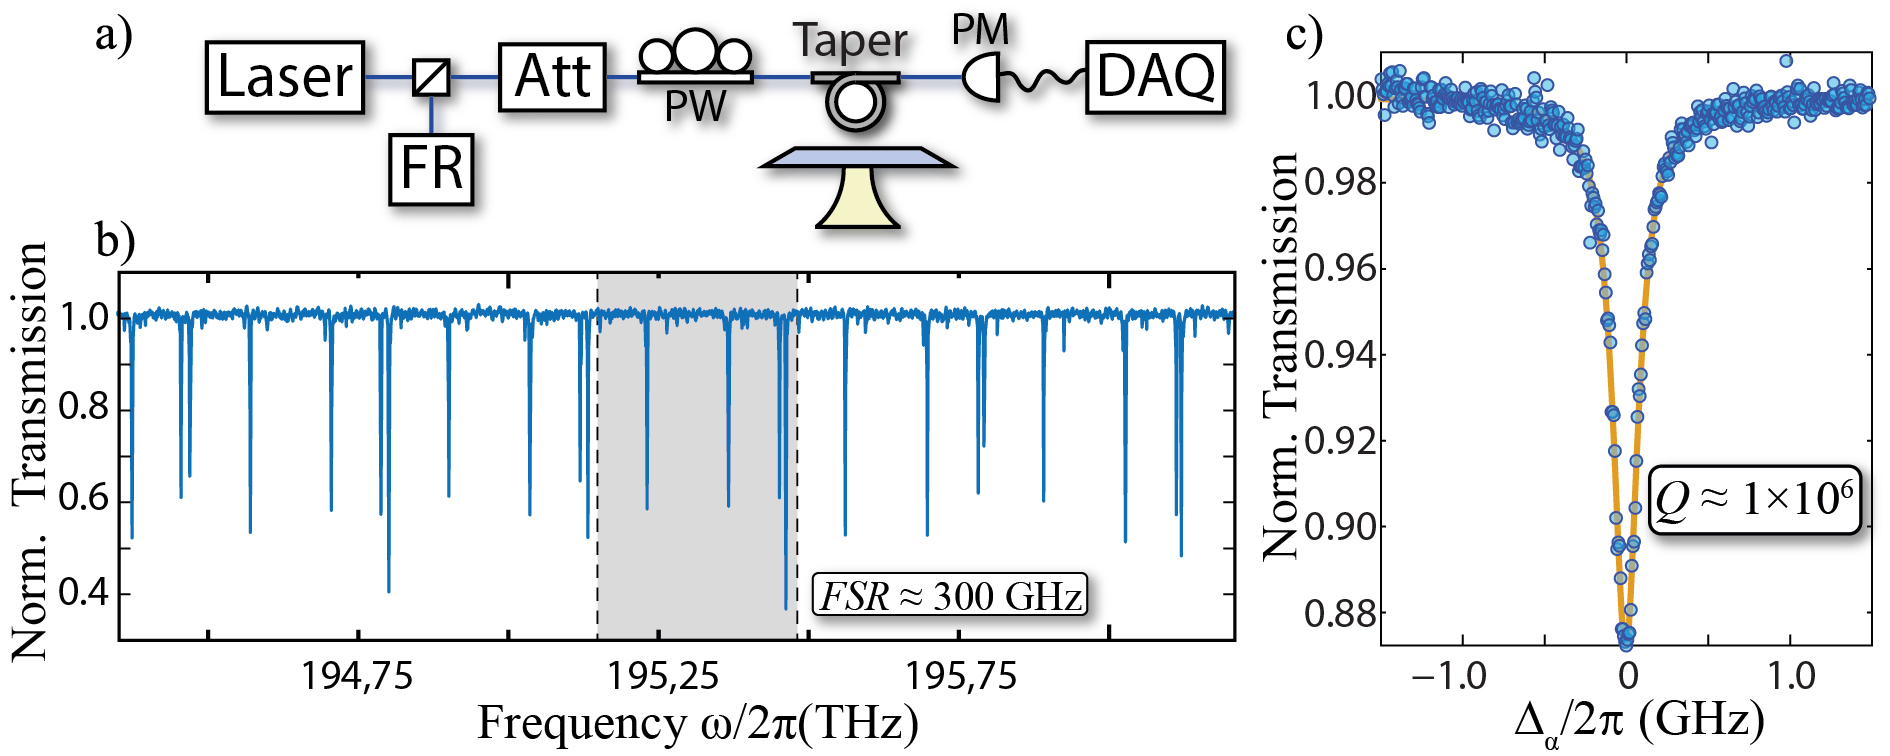
\includegraphics[width = 16cm]{figuras/Dissertation_optical_char_exp.jpg}
    \caption{Caption}
    \label{fig:exp_mode_charac}
\end{figure}

The result, for a single mode, are presented in the Fig~\ref{fig:exp_mode_charac}b). We use the Eq~\ref{eq:single_mode_transmission} to fit the data giving the values of $300$ MHz and $50$ MHz for the $\kappa_j^{(i)}$ and $\kappa_j^{(e)}$, respectively. The mode are at frequency $\omega_j = 2\pi\times195.25$ THz which give us a $Q \approx 2\times10^6$.

%The same setup are used
Using an stepper motor instead of the piezo it possible to modulate the frequency in few THz enabling us to measure different families of modes, as show in Fig~\ref{fig:exp_mode_charac}c). The spectral distance of a mode in consecutive families give the $FSR_j$ for the $j$ mode. 









